\documentclass{article} % For LaTeX2e
\usepackage{nips14submit_e,times}
\usepackage{amsmath}
\usepackage{amsthm}
\usepackage{amssymb}
\usepackage{mathtools}
\usepackage{hyperref}
\usepackage{url}
\usepackage{algorithm}
\usepackage[noend]{algpseudocode}
%\documentstyle[nips14submit_09,times,art10]{article} % For LaTeX 2.09

\usepackage{bbm}
\usepackage{graphicx}
\usepackage{caption}
\usepackage{subcaption}
\usepackage{MnSymbol}

\def\eQb#1\eQe{\begin{eqnarray*}#1\end{eqnarray*}}
\def\eQnb#1\eQne{\begin{eqnarray}#1\end{eqnarray}}
\providecommand{\e}[1]{\ensuremath{\times 10^{#1}}}
\providecommand{\pb}[0]{\pagebreak}
\DeclarePairedDelimiter\ceil{\lceil}{\rceil}
\DeclarePairedDelimiter\floor{\lfloor}{\rfloor}

\newcommand{\E}{\mathrm{E}}
\newcommand{\Var}{\mathrm{Var}}
\newcommand{\Cov}{\mathrm{Cov}}
\newcommand\eqD{\stackrel{\mathclap{\normalfont\mbox{d}}}{=}}

\def\Qb#1\Qe{\begin{question}#1\end{question}}
\def\Sb#1\Se{\begin{solution}#1\end{solution}}

\newenvironment{claim}[1]{\par\noindent\underline{Claim:}\space#1}{}
\newtheoremstyle{quest}{\topsep}{\topsep}{}{}{\bfseries}{}{ }{\thmname{#1}\thmnote{ #3}.}
\theoremstyle{quest}
\newtheorem*{definition}{Definition}
\newtheorem*{theorem}{Theorem}
\newtheorem*{lemma}{Lemma}
\newtheorem*{question}{Question}
\newtheorem*{preposition}{Preposition}
\newtheorem*{exercise}{Exercise}
\newtheorem*{challengeproblem}{Challenge Problem}
\newtheorem*{solution}{Solution}
\newtheorem*{remark}{Remark}
\usepackage{verbatimbox}
\usepackage{listings}
\usepackage{mathrsfs}
\title{ProbLimI: \\
Problem Set X}


\author{
Youngduck Choi \\
CIMS \\
New York University\\
\texttt{yc1104@nyu.edu} \\
}


% The \author macro works with any number of authors. There are two commands
% used to separate the names and addresses of multiple authors: \And and \AND.
%
% Using \And between authors leaves it to \LaTeX{} to determine where to break
% the lines. Using \AND forces a linebreak at that point. So, if \LaTeX{}
% puts 3 of 4 authors names on the first line, and the last on the second
% line, try using \AND instead of \And before the third author name.

\newcommand{\fix}{\marginpar{FIX}}
\newcommand{\new}{\marginpar{NEW}}

\nipsfinalcopy % Uncomment for camera-ready version

\begin{document}


\maketitle

\begin{abstract}
This work contains solutions to the exercises of the problem set X. The
chosen problems are 2,3,4.
\end{abstract}

\bigskip


\begin{question}[2]
\end{question}
\begin{solution} \hfill \\
\textbf{(a)}
Observe that
\eQb
\mathbb{P}(y_{n+1} = 1 | y_1 = i, ...,  y_{n} = i_n ) &=& 
\dfrac{\int_{0}^{1} z^{n+1} (1-z)^{n-N} dz}{\int_{0}^{1} z^n (1-z)^{n-N} dz}
= \dfrac{N+1}{N+2} = \dfrac{S_n + n + 2}{2n + 4} 
\eQe
so 
\eQb
\mathbb{P}(S_{n+1} = s| \mathscr{F}_n) \in \sigma(S_n)
\eQe
and 
\eQb
\mathbb{P}(S_{n+1} = s | \mathscr{F}_n) = \mathbb{P}(S_{n+1} = s| s_n).
\eQe
Therefore, $\{S_n\}$ is a Markov chain.

\textbf{(b)} From the above formula, the transition probability is 
$\dfrac{n - x -2}{2n+4}$ if $y = x-1$, $\dfrac{n+x+2}{2n+4}$ if  $y = x+1$,
and $0$ otherwise. 

\textbf{(c)} Not homogeenous, as the transition probability depends on $n$.
\hfill $\qed$

\end{solution}

\newpage

\begin{question}[2]
\hfill
\begin{figure}[h!]
  \centering
    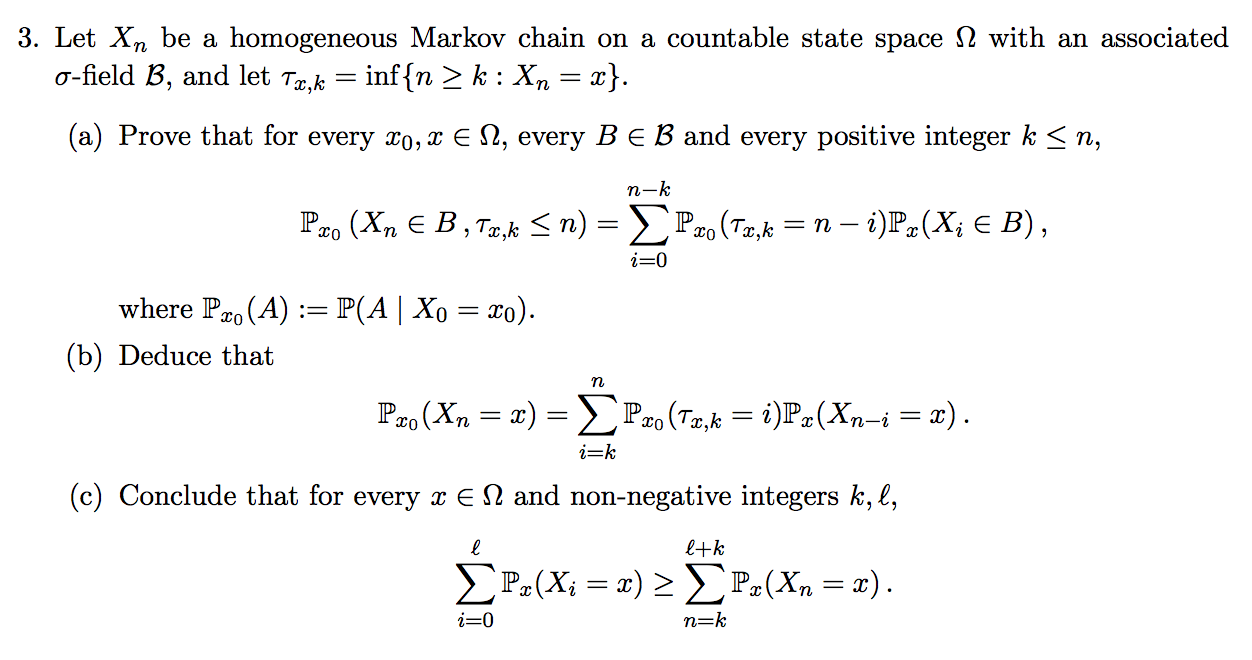
\includegraphics[width=0.7\textwidth]{prob-e10-p2.png}
\end{figure}
\end{question}
\begin{solution} \hfill \\
\textbf{(a)} 
By homogeneity,
\eQb
\mathbb{P}_x(X_i \in B) = 
\mathbb{P}(X_i \in B | X_0 = x) = \mathbb{P}(X_n \in B | X_{n-i} = x) 
\eQe
for any $1 \leq i \leq n$. Then, 
\eQb
\mathbb{P}_{x_0}(X_n \in B , \tau_{x,k} \leq n) &=& 
\mathbb{P}_{x_0}(\bigcup_{i=0}^{n-k} X_n \in B , \tau_{x,k} = n-i) \\
&=& \sum_{i=0}^{n-k} \mathbb{P}_{x_0}( X_n \in B , \tau_{x,k} = n-i) \\
&=&
\sum_{i=0}^{n-k} \mathbb{P}_{x_0}(\tau_{x,k} = n-i)\mathbb{P}(X_n \in B | X_{n-i} = x)
\\ 
&=& 
\sum_{i=0}^{n-k} \mathbb{P}_{x_0}(\tau_{x,k} = n-i)\mathbb{P}_{x}(X_i \in B). 
\eQe

\bigskip

\textbf{(b)} In view of (a), setting $B = \{x\}$,
\eQnb
\mathbb{P}_{x_0}(X_n = x)
&=& \mathbb{P}_{x_0}(X_n = x, \tau_{x,k} \leq n) \label{eq:1} \\
&=& \sum_{i=k}^{n} 
\mathbb{P}_{x_0}(\tau_{x,k} = i)\mathbb{P}_x(X_{n-i} = x) \nonumber 
\eQne
where~\eqref{eq:1} holds as $\{X_n = x\} \subset \{ \tau_{x,k} \leq n \}$. 

\bigskip

\textbf{(c)} Applying (b) with $x_0 = x$,  
\eQnb
\sum_{n=k}^{l+k} \mathbb{P}_x(X_n = x) &=& 
\sum_{n=k}^{l+k} \sum_{i=k}^{n} \mathbb{P}_x(\tau_{x,k} = i) 
\mathbb{P}_x(X_{n-i} = x) \nonumber \\ 
&=& \sum_{i=0}^{l} \mathbb{P}_x( X_i = x) \sum_{i=k}^{n-j} \mathbb{P}_x(
\tau_{x,k} = i) \nonumber \\
&\leq& \sum_{i=0}^{l} \mathbb{P}_x( X_i = x) \label{eq:3} 
\eQne
where~\eqref{eq:3} holds by disjointness. \hfill $\qed$ 

\end{solution}

\newpage

\begin{question}[3]
\hfill
\begin{figure}[h!]
  \centering
    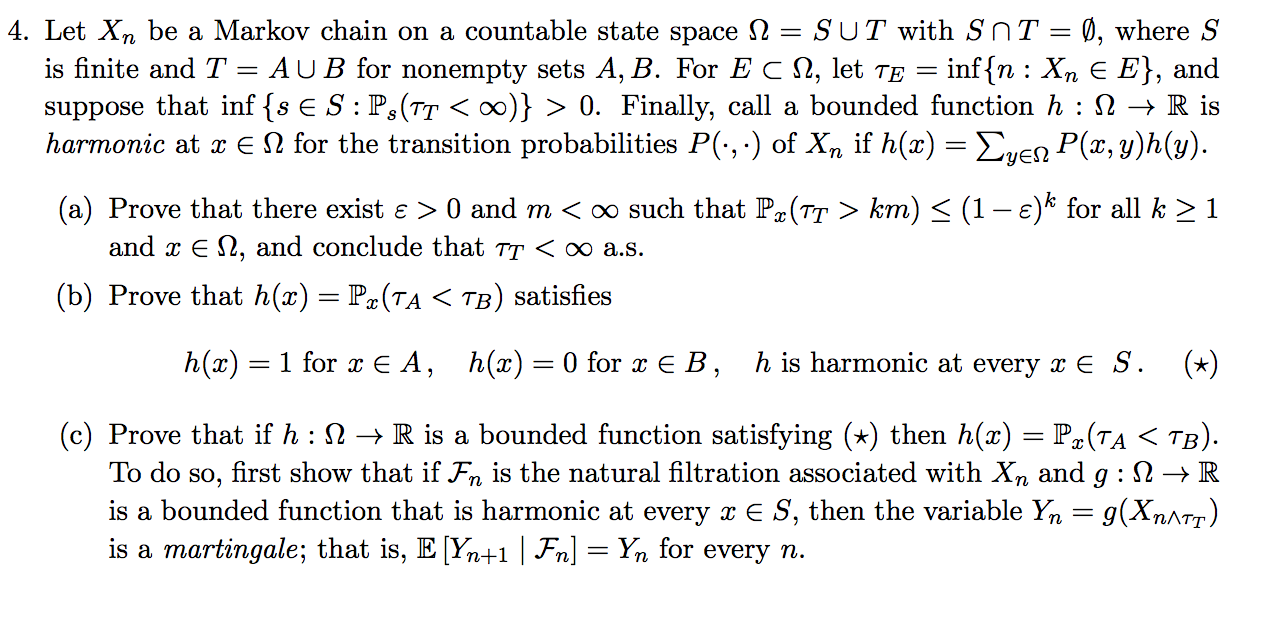
\includegraphics[width=0.7\textwidth]{prob-e10-p3.png}
\end{figure}
\end{question}
\begin{solution} \hfill \\
\textbf{(a)} 
Denote $\theta_k$ as a shift operator of the chain. As $S$ is finite,
choose $m$ such that $\epsilon = \min_{s \in S} \mathbb{P}_s(\tau_T \leq m) > 0$.
Then, with $k \geq 2$,
\eQb
\mathbb{P}_s(\tau_T > km) &=& \mathbb{P}_s(\tau_T > (k-1)m, \tau_T \circ \theta_{
(k-1)m} > m) \\
&=& \mathbb{E}_s(\mathbb{P}_s \circ \theta_{(k-1)m} > m | \mathscr{F}_{(k-1)m} 
1_{\{\tau_T > (k-1)m\}}) \\
&\leq&\mathbb{P}_s(\tau_T > (k-1)m) 
\eQe
where the last inequality holds by Markov property. $k=1$ is obvious, so
by induction we are done. By summability, $\tau_{T}m^{-1} < \infty$
almost surely, so $\tau_{T} < \infty$ almost surely.


\bigskip

\textbf{(b)} If $x \in A$, then
\eQb
\tau_{A} = 0 \>\>\> \text{and} >\>\> 
\tau_{B} \geq 1 \>\>\> \mathbb{P}_x \>\>\> \text{almost surely}, 
\eQe
and hence $h(x) = \mathbb{P}_x(\tau_A < \tau_B) = 1$ for $x \in A$. Similarly,
$h(x) = 0$ for $x \in B$. 

for any $x \in S$. Suppose $x \not\in T$. Then,
\eQb
1_{\tau_{A} < \tau_{B}} \circ \theta_1 = 1_{\tau_B < \tau_B}
\eQe
and hence
\eQb
\mathbb{E}_X(\tau_{A} < \tau_B) = \mathbb{E}_X(\mathbb{P}_{X_1}(\tau_A < \tau_B))
= \mathbb{E}_{X}[h(x_1)].
\eQe
Therefore $h$ is harmonic.


\bigskip

\textbf{(c)} Fix $n \geq 1$, and $E \in \mathscr{F}_n$.
By definition of conditional expectation, we wish to show
\eQb
\int_{E} Y_{n+1} = \int_{E} Y_n 
\eQe
which can be rewritten as
\eQb
\int_{E \cap \{\tau_T \leq n\}} Y_{n+1}  \int_{E \cap \{ \tau_T > n\}} 
Y_{n+1} 
&=& \int_{E \cap \{\tau_T \leq n\}} Y_{n} +  \int_{E \cap \{ \tau_T > n\}}  
Y_{n} 
\eQe
Observe that 
\eQb
Y_{n+1} = Y_{n} \>\>\> \text{on} \>\>\> \{\tau_T \leq n \} 
\eQe
as well as
\eQb
Y_{n+1} = g(X_{n+1}) \>\>\> \text{and} \>\>\> 
Y_{n} = g(X_n) \>\>\> \text{on} \>\>\> \{\tau_T > n \}. 
\eQe
Therefore, it suffices to show that
\eQb
\int_{E \cap \{ \tau_T > n\}} 
g(X_{n+1}) 
&=& 
\int_{E \cap \{ \tau_T > n\}}  
g(X_n). 
\eQe

Now, by harmonic,
\eQb
\sum_{\omega \in \Omega} \mathbb{P}(s,\omega) X_n(\omega) = X_n(s) 
\eQe

and
\eQb
\sum_{s \in S} \int_{E \cap \{ X_n = s\} } g(X_{n+1}) &=& 
\sum_{s \in S} \int_{E \cap \{ X_n = s\} } g(X_{n})  
\eQe
By harmonic 
\eQb
\sum_{s \in S} \int_{E \cap \{ X_n = s\} } g(X_{n+1}) &=&
\sum_{s \in S} X_n(s) \mathbb{P}(A_s)   
\eQe
and 
\eQb
\sum_{s \in S} \int_{E \cap \{ X_n = s\} } g(X_{n+1}) &=& 
\sum_{s \in S} X_n(s) \mathbb{P}(A_s)   
\eQe


\end{solution}
\end{document}


